% ---------------------------------------------------------------------
% HEADER
% Formålet med å legge header til et eget dokument er å garantere at
% oppsettet av dokumentene er likt for alle løsningsforslagene.
% I headeren skjer følgende:
% (1) Dokumentet blir startet
% (2) Pakker blir importert
% ---------------------------------------------------------------------
% ---------------------------------------------------------------------
% HEADER
% Formålet med header er å importere de samme pakkene i alle dokumentene.
% ---------------------------------------------------------------------

% Sett opp dokumentet. Her kan 'twoside' brukes for printing
\documentclass[12pt, a4paper]{article}

% Vi trenger utf-8 for å bruke norske bokstaver: Æ, Ø, Å
\usepackage[utf8]{inputenc}

% Vi setter babel til norsk, da får dokumentegenskaper norske titler
\usepackage[norsk]{babel}

% For å kunne bruke grafikk
\usepackage{graphicx}
\newcommand{\figwidth}{0.75}

% Matematikkpakker fra AMS - American Mathematical Society
\usepackage{amsmath, amsthm, amsfonts, amssymb, mathtools}

% For eventuelle linker, e.g. \href{URL}{text}
\usepackage{hyperref}

% For headers og footers med eventuell logo
\usepackage{fancyhdr}

% Sett marginer manuelt
\usepackage[top = 3cm, left = 3cm, right = 3cm, bottom = 3cm]{geometry}

% For enkle lister, nyttig for oppgave a), b), c), ...
\usepackage[sharp]{easylist}

% Dersom flere kolonner er ønskelig i deler av dokumentet
\usepackage{multicol}

% For luft mellom paragrafer
\usepackage{parskip}

% For logikk assosiert med logoer
\usepackage{ifthen}

% For å finne totalt antall sider
\usepackage{lastpage}

% Annet
\usepackage{enumitem}

\usepackage{polynom}% Polynomer
\polyset{style=C, div=:}

\usepackage{systeme}% Likningssystemer

% Kan brukes når noe stryker ut noe, f.eks 1/n * n, her kan man ta \frac{1}{\cancel{n}} * \cancel{n}
\usepackage{cancel}



% ---------------------------------------------------------------------
% DOKUMENTVARIABLER
% ---------------------------------------------------------------------
\newcommand{\fagkode}{S2}
\newcommand{\semesteraar}{høsten 2015}
\newcommand{\forfatter}{Tommy O.}
\newcommand{\dokumenttittel}{Løsningsforslag -- Eksamen \fagkode, \semesteraar}


% Set til 'true' og oppgi logo dersom du vil bruke en logo
\newboolean{bruklogo}
\setboolean{bruklogo}{false}
\newcommand{\logonavn}

% ---------------------------------------------------------------------
% SETUP
% Formålet med å legge setup til et eget dokument å garantere at headers,
% footers, og øverste del av dokumentet er likt for alle
% løsningsforslagene.
% ---------------------------------------------------------------------
% ---------------------------------------------------------------------
% HEADER
% Formålet med setup er at dokumentene ser rimelig like ut.
% ---------------------------------------------------------------------


% ---------------------------------------------------------------------
% Alternativ font. Kommentert ut fordi Computer Modern (default) er pen
%\usepackage{kmath,kerkis}
%\usepackage[T1]{fontenc}
% ---------------------------------------------------------------------


% ---------------------------------------------------------------------
% Sett opp headers og footers
\ifthenelse{\boolean{bruklogo}}{
% Dersom logo skal brukes, sett logoen oppe til høyre med bredde 4 cm
	\rhead{\includegraphics[width=3.5cm]{\logonavn}}
}{
% Dersom logo ikke skal brukes, sett tom header
	\rhead{}
} 
\rfoot{\thepage}
\cfoot{}
\lhead{}
\lfoot{{\scriptsize Forbedringsforslag? Bidra på \url{https://github.com/tommyod/matte_eksamener_VGS}.}}
\renewcommand{\headrulewidth}{0pt}
% ---------------------------------------------------------------------


% ---------------------------------------------------------------------
% To streker under svaret
\def\answer#1{\underline{\underline{#1}}}
% ---------------------------------------------------------------------


% ---------------------------------------------------------------------
% Start selve dokumentet
% ---------------------------------------------------------------------

\begin{document}
\pagestyle{fancy}
{\bfseries \Large \dokumenttittel} \\
{ \footnotesize Laget av \forfatter 
	\hfill Sist oppdatert: \today 
	\hfill Antall sider: \pageref*{LastPage}}
\hrule
\vspace{1em}
\begin{center}
\fbox{\fbox{\parbox{.90\textwidth}{
	Dette dokumentet er open-source;
	alle kan bidra til å gjøre det bedre.
	Dersom du finner skrivefeil, matematiske feil, eller ser at forklaringene kan være bedre: ikke nøl med å sende inn en endring. 
	Du kan finne siste versjon, og bidra, på GitHub, se:
	\url{https://github.com/tommyod/matte_eksamener_VGS}
}}}
\end{center}


% ---------------------------------------------------------------------
% DOKUMENTSTART - Skriv løsningsforslaget nedenfor
% ---------------------------------------------------------------------	
\section*{Del 1 - uten hjelpemidler}
\subsection*{Oppgave 1}
\begin{easylist}[enumerate]
	\ListProperties(Style2*=,Numbers=a,Numbers1=l,FinalMark={)})
	# Vi skal derivere funksjonen $f(x) = x^3 + 2x$.
	Formelen vi må bruke er $(x^n)' = nx^{n-1}$, og vi får $f'(x) = \left(x^3\right)' + \left(2x\right)' = \answer{3x^2 + 2}$ som svar.

	# Neste funksjon er $g(x) = 3e^{2x-1}$.
	Kjerneregelen sier at dersom $f = e^{u(x)}$, så er $f' = e^{u(x)} u'(x)$.
	Vår $u(x)$ er $ 2x-1$, slik at vi får $f'(x) = 3e^{2x-1} (2x-1)' = 3e^{2x-1} 2 = \answer{6e^{2x-1}}$.
	
	# Tredje og siste funksjon er $h(x) = x^2e^x$.
	Denne er kanskje litt vanskeligere. Funksjonen er et produkt av to funksjoner som vi vet hvordan vi  kan derivere, nemlig $u = x^2$ og $u = e^x$.
	Produktregelen sier at $(uv)' = u'v + uv'$. Ved å bruke produktregelen får vi
	\begin{align*}
		h'(x) &= \left(x^2\right)'  e^x + x^2\left(e^x\right)' \\
			&= 2x  e^x + x^2e^x \\
			&= \answer{xe^x\left(x+2\right)}.
	\end{align*}
\end{easylist}

\subsection*{Oppgave 2}
Vi skal her se på funksjonen 
\begin{equation*}
	f(x) = x^3 + 3x^2 - 9x.
\end{equation*}
\begin{easylist}[enumerate]
	\ListProperties(Style2*=,Numbers=a,Numbers1=l,FinalMark={)})
	# Den deriverte er $f'(x) = 3x^2 + 6x - 9 = 3(x^2 + 2x - 3)$.
	Vi kan faktorisere ved inspeksjon eller ved hjelp av ABC-formelen.
	Vi setter den deriverte lik null, og får da $f'(x) = 3(x+3)(x-1) = 0$, 
	slik at $x = 1$ og $x = -3$ gir $f'(x) = 0$.
	Vi kan bruke den andrederiverte til å karakterisere punktene,
	så vi regner det ut med en gang. Den andrederiverte blir $f''(x) = 6x+6$.
	
	## Når $x =1$ er $f(1) = (1)^3 + 3(1)^2 - 9(1) = -5$.
	Punktet er et bunnpunkt fordi $f''(1) = 12 > 0$.
	Punktet \answer{$(1, f(1)) = (1, -5)$ er et bunnpunkt}.
	## Når $x =-3$ er $f(-3) = (-3)^3 + 3(-3)^2 - 9(-3) = 27$.
	Denne gangen er punktet et toppunkt, fordi $f''(-3) = -12 < 0$. \\
	Punktet \answer{$(-3, f(-3)) = (-3, 27)$ er et toppunkt}.
	
	# Et vendepunkt oppstår når $f''(x) = 6x+6 = 6(x+1)$ endrer fortegn,
	dette skjer når $x = -1$. Punktet \answer{$(-1, f(-1)) = (-1, 11)$ er et vendepunkt}.
	
	# På figur \ref{fig:del12cplot} ser du en et plot av $f(x)$ og $f'(x)$.
	Med kunnskap om bunnpunkt, toppunkt og vendepunkt bør det ikke være vanskelig å lage en skisse for hånd også.
	\begin{figure}[th!]
		\centering
		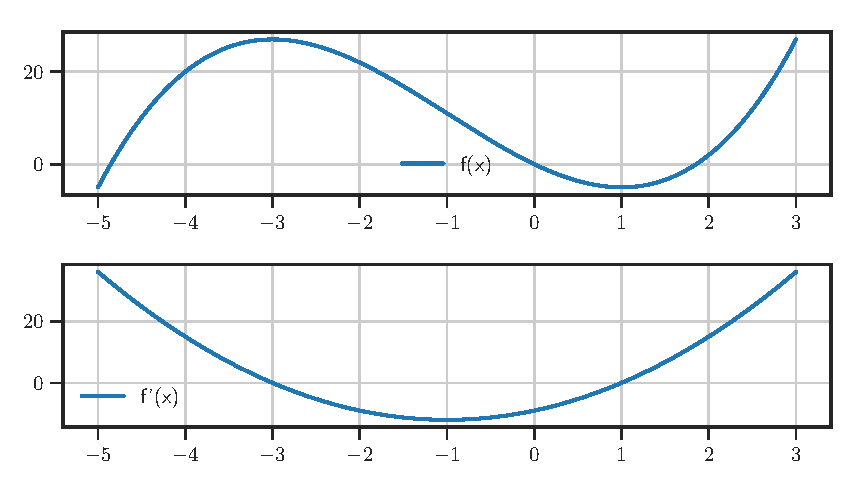
\includegraphics[width=0.7\linewidth]{figs/del1_2c_plot}
		\caption{Funksjonen $f(x) = x^3 + 3x^2 - 9x$ i oppgave 2, del 1.}
		\label{fig:del12cplot}
	\end{figure}
\end{easylist}

\subsection*{Oppgave 3}
\begin{easylist}[enumerate]
	\ListProperties(Style2*=,Numbers=a,Numbers1=l,FinalMark={)})
	# Vi har et polynom $p(x) = x^3 - ax^2 + 2ax - 8$, og vi skal vise at det er delelig
	med $(x-2)$ for alle verdier av $a$. Husk at generelt er et polynom $f(x)$ delelig med $(x-b)$ dersom $p(b) = 0$. I vårt tilfelle er $b = 2$, så vi sjekker $p(2)$ og får
	\begin{align*}
		p(2) &= (2)^3 - a(2)^2 + 2a(2) - 8 \\
		&= 8 - 4a + 4a - 8 \\
		&= \answer{a(4-4) = 0}.
	\end{align*}
	Polynomet er altså delelig med $(x-2)$ for alle verdier av $a$, slik som oppgaven ba oss om å vise.
	
	# Telleren i brøken er $p(x)$ i forrige oppgave med $a = 1$, så vi vet allerede at divisjonen går opp.
	Bruk polynomdivisjon, du skal få \answer{$x^2 + x + 4$} som svar. 
\end{easylist}

\subsection*{Oppgave 4}
Vi skal løse følgende likningssystem, og vi skal legge sammen og trekke likninger fra hverandre for å finne en løsning.
\begin{align*}
	\mathbf{L1: }\quad &x + 2y - z = 2\\
	\mathbf{L2: }\quad &2x - y + z = 3 \\
	\mathbf{L3: }\quad &3x - 2y + 2z = 2
\end{align*}
Det er lurt å kikke litt på likningene før vi begynner å løse, for å prøve å finne en effektiv fremgangsmåte.
Vi ser at koeffisientene foran $y$ og $z$ i $\mathbf{L2}$ og $\mathbf{L3}$ er veldig like.
Vi tar $2 \times \mathbf{L2} - \mathbf{L3}$ og finner at $x = 4$. 
Når vi setter $x = 4$ inn i likningene\footnote{Vi har brukt $\mathbf{L2}$ og $\mathbf{L3}$, så vi må bruke $\mathbf{L1}$ videre. Vi kan velge å sette inn i  $\left\{\mathbf{L2}, \mathbf{L1}\right\}$ eller $\left\{\mathbf{L3}, \mathbf{L1}\right\}$. Vi kommer oss videre og får det samme likningssystemet etter innsetting uansett, sjekk gjerne dette om du ikke tror det.} får vi 2 nye likninger.
\begin{align*}
\mathbf{L4: }\quad &2y - z = -2\\
\mathbf{L5: }\quad &- y + z = -5
\end{align*}
Dersom vi tar $\mathbf{L4} + \mathbf{L5}$ blir vi kvitt $z$ og ser at $y = -7$.
Deretter er det bare å sette inn $y = -7$ i $\mathbf{L4}$ eller $\mathbf{L5}$ og løse for $z$,
da finner vi ut at $z = -12$. Vi har løst likningssystemet, og ser at \answer{løsningen blir $x = 4$, $y = -7$ og $z = -12$}. Det er lurt å sette prøve på svaret når man løser slike oppgaver på eksamen.

\subsection*{Oppgave 5}
Vi ser på rekken
\begin{equation*}
	\underset{a_1}{\underbrace{1}} + \underset{a_2}{\underbrace{\frac{1}{2}}} + \underset{a_3}{\underbrace{\frac{1}{4}}} + ... + \underset{a_n}{\underbrace{\frac{1}{2^{n-1}}}}.
\end{equation*}
\begin{easylist}[enumerate]
	\ListProperties(Style2*=,Numbers=a,Numbers1=l,FinalMark={)})
	# Dette er en geometrisk rekke fordi \answer{kvotienten $k = a_i / a_{i-1}$ er konstant} for alle verdier av $i$.
	Med andre ord kan vi ta et hvilket som helst ledd og gange med $k$ for å få det neste leddet. I denne oppgaven ser vi at
	$k = 1/2$ ved å f.eks. regne ut $k = a_2 / a_{1} = (1/2)/1 = 1/2$.
	
	For å finne summen må vi bruke summeformelen for geometriske rekker. 
	Summen av de $n$ første leddene er gitt ved formelen
	\begin{equation}
	\label{eqn:5a}
		S_n = a_1 \times \frac{1-k^n}{1-k} = 1 \times \frac{1-(1/2)^n}{1-(1/2)} = \answer{2 \left( 1-\frac{1}{2^n} \right)}.
	\end{equation}
	Vi bør sjekke at svaret stemmer for noen enkle summer som $S_1 = a_1$, $S_2 = a_1 + a_2$, og så videre.
	
	# Her kan vi bruke formelen for summen av en uendelig geometrisk rekke
	\begin{equation*}
		S = \frac{a_1}{1 - k} = \frac{1}{1 - (1/2)} = \answer{2}.
	\end{equation*}
	Alternativt kan vi la $n$ gå mot uendelig i likning \eqref{eqn:5a}, da får vi
	\begin{equation*}
		\lim_{n \to \infty } 2 \left( 1-\frac{1}{2^n} \right)= 2 \left( 1-0 \right) = \answer{2}.
	\end{equation*}
\end{easylist}

\subsection*{Oppgave 6}
\begin{easylist}[enumerate]
	\ListProperties(Style2*=,Numbers=a,Numbers1=l,FinalMark={)})
	# De fire første leddene blir:
	\begin{align*}
		a_1 &= (1)^3 + 1 = 2   \\
		a_2 &= (2)^3 + 1 = 9   \\
		a_3 &= (3)^3 + 1 = 28   \\
		a_4 &= (4)^3 + 1 = 65   
	\end{align*}
	
	# Å vise delelighet er enkelt og greit:
	\begin{align*}
	a_1 &= (1)^3 + 1 =2 \ \rightarrow \ 2 / 2 =1  \\
	a_2 &= (2)^3 + 1 =9 \ \rightarrow \ 9  / 3 = 3 \\
	a_3 &= (3)^3 + 1 =28 \ \rightarrow \ 28  / 4 = 7 \\
	a_4 &= (4)^3 + 1 =65 \ \rightarrow \ 65   / 5 = 13
	\end{align*}
	
	# Dersom $a_n = n^3 + 1$ er delelig med $(n+1)$ så må $(n+1)$ være en faktor,
	altså kan vi skrive $a_n = (n+1) p_2(n)$, der $p_2(n)$ er et andregradspolynom i variabelen $n$.
	Vi kan sjekke at $(n+1)$ er en faktor ved å se at $a_{-1} = (-1)^3 + 1 = 0$.
	Legg merke til hvor likt dette er situasjonen med polynomer.
	Vi kan finne $p_2(n)$ ved å utføre polynomdivisjonen $(n^3  + 0n^2 + 0n+ 1):(n+1)$, vi får da at $p_2(n) = n^2 -n + 1$.
	\begin{equation*}
		\answer{a_n = n^3 + 1 = (n^2 -n + 1)(n+1) = \text{delelig med }(n+1)}
	\end{equation*}
\end{easylist}

\subsection*{Oppgave 7}
\begin{easylist}[enumerate]
	\ListProperties(Style2*=,Numbers=a,Numbers1=l,FinalMark={)})
	# Inntekten er prisen per enhet ganget med antall enheter.
	\begin{equation*}
		I(x) = p(x) \times x = \left(480 - 0.1x\right)x = \answer{480x - 0.1x^2}
	\end{equation*}
	# Overskuddet er inntekten minus kostnaden.
	\begin{align*}
		O(x) &= I(x) - K(x) \\
		&= \left[ 480x - 0.1x^2 \right] - \left[20000+120x + 0.05x^2\right] \\
		&= \answer{-0.15x^2 + 360x - 20000}
	\end{align*}
	Dersom $O'(x^*) = 0$ har vi minimumspunkt, maksimumspunkt eller terrassepunkt i punktet $x^*$.
	Vi regner ut den førstederiverte og andrederiverte.
	\begin{align*}
		O'(x) &= -0.3x + 360 \\
		O''(x) &= -0.3
	\end{align*}
	Vi ser at $O'(x^*) = 0 \Rightarrow -0.3x^* + 360 = 0 \Rightarrow  \answer{x^* = 1200}$. Dett er et maksimumspunkt fordi $O''(x^*)$ er negativ.\footnote{Funksjonen $f(x) = ax^2 + bx + c$ har maksimum når $a < 0$ og minimum når $a > 0$.}
	
\end{easylist}

\subsection*{Oppgave 8}
\begin{easylist}[enumerate]
	\ListProperties(Style2*=,Numbers=a,Numbers1=l,FinalMark={)})
	# I matematikk er det alltid lurt å lage en tegning eller tabell om du har mulighet.
	Vi lager en tabell som viser de 2 terningene og summen.
	\begin{center}
		\begin{tabular}{c|cccccc}
			& \textbf{1} & \textbf{2} & \textbf{3} & \textbf{4} & \textbf{5} & \textbf{6}  \\ \hline
		  \textbf{1} & 2 & 3 & 4 & 5 & 6 & 7  \\
		  \textbf{2} & 3 & 4 & 5 & 6 & 7 & 8  \\
		  \textbf{3} & 4 & 5 & 6 & 7 & 8 & 9  \\
		  \textbf{4} & 5 & 6 & 7 & 8 & 9 & 10  \\
		  \textbf{5} & 6 & 7 & 8 & 9 & 10 & 11  \\
		  \textbf{6} & 7 & 8 & 9 & 10 & 11 & 12  
		\end{tabular}
	\end{center}
	Når $x = a-200$ må kasinoet betale ut 200 kroner. Dette skjer når summen er 10, og antall måter dette kan skje på er 3 (se tabellen ovenfor). Derfor blir $P(X = a - 200) = 3 / 36 = 1/12$.
	På samme måte er sjansen for at kasinoet må betale ut 50 kroner lik $P(X = a - 50) = 6 / 36 = 1/6$.
	Vi fyller ut tabellen slik:
\begin{center}
	\begin{tabular}{|c|c|c|c|}
		\hline
		$x$ & $a$ & $a-200$ & $a-50$ \\ \hline
		$P(X = x)$ & $27 / 36$ & \answer{$3/36 = 1/12$} & \answer{$6/36 = 1/6$} \\ \hline
	\end{tabular}
\end{center}
	Selv om det er god skikk å forkorte brøker er det lettere å se at summen av sannsynlighetene blir 1 dersom vi ikke gjør det---dette er en viktig sjekk for å se at vi har regnet riktig.
	
	# Forventet gevinst skal være 5, så vi setter $\operatorname{E}(X) = 5$ og løser for $a$:
	\begin{align*}
		\operatorname{E}(X) = \sum_{x \in X} x P(X = x) &= 5 \\
		 a\frac{27}{36} + (a-200)\frac{3}{36}+ (a-50)\frac{6}{36} &= 5 \\
		a27 + (a-200)3 + (a-50)6 &= 180 \\
		36a &= 180 + 900 \\
		a &= \frac{1080}{36} = \frac{540}{18} = \frac{270}{9} \\
		a &= \answer{30} 
	\end{align*}
	Kasinoet må sette prisen til 30 kroner. En simulering av dette kasinoet for 2000 spill finner du i figur \ref{fig:del18plot}. Kasinoet har kanskje ikke så god profitt i starten, men over tid er det helt klart at kasinoet er vinneren.
	
	\begin{figure}[th!]
		\centering
		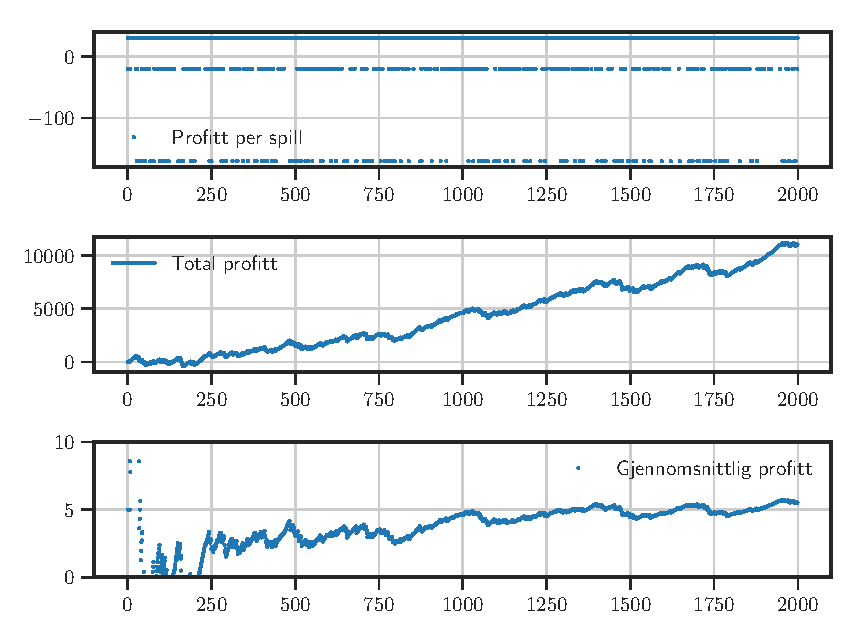
\includegraphics[width=0.85\linewidth]{figs/del1_8_plot}
		\caption{Simulering av kasinoet med $a = 30$ i oppgave 8, del 1.}
		\label{fig:del18plot}
	\end{figure}
\end{easylist}

\subsection*{Oppgave 9}
\begin{easylist}[enumerate]
	\ListProperties(Style2*=,Numbers=a,Numbers1=l,FinalMark={)})
	# Vi har at $X \sim \mathcal{N}(\mu = 2000, \sigma = 400)$. Sannsynligheten for at en tilfeldig valgt lyspære lyser i færre enn 1600 timer er $P(X \leq 1600)$. Vi transformerer problemet til standardnormalfordelingen ($\mathcal{N}(\mu = 0, \sigma = 1)$) slik som dette:
	\begin{equation*}
		P(X \leq 1600) =P\left(\frac{X-\mu}{\sigma} \leq \frac{1600-2000}{400} \right) = P(Z \leq -1)
	\end{equation*}
	Fra tabellen i vedlegg 1\footnote{Tabell for standard normalfordeling.} leser vi av at $P(Z \leq -1) = \answer{0.1587}$.
	
	#  Oppgaven spør ``for hvilken verdi $x$ har vi at $P(X > x) = 0.9$?'' 
	Vi vet at $P(X \leq x) + P(X > x) = 1$ fordi summen av sannsynligheten alltid er 1, så vi har at
	\begin{equation*}
		P(X \leq x) + 0.9 = 1 \Rightarrow P(X \leq x) = 0.1.
	\end{equation*}
	Dette kan vi finne ved hjelp av tabellen vår. Vi gjør om til standard normalfordeling:
	\begin{equation*}
		P(X \leq x) = 0.1 \Leftrightarrow P\left(\frac{X-\mu}{\sigma} \leq \frac{x-\mu}{\sigma}\right) = 0.1 \Leftrightarrow P(Z \leq z) = 0.1
	\end{equation*}
	Fra tabellen ser vi at $P(Z \leq -1.28) \approx 0.1$, dette er nøyaktig nok for vårt formål.
	Vi må transformere tilbake til $x$, så vi snur på formelen:
	\begin{equation*}
		z = \frac{x - \mu}{\sigma} \ \Leftrightarrow \ x = \mu + z \sigma
	\end{equation*}
	Må må vi regne ut $x$ gitt $z$. Legg merke til hvordan vi kan regne dette ut uten kalkulator.
	\begin{align*}
		x &= \mu + z \sigma \\
		  &= 2000 + (-1.28) 400 \\
		  &= 2000 - (1+0.2 + 0.08)400 \\
		  &= 2000 - 400 - 80 - 32 \\
		  &= 2000 - 512 = \answer{1488}
	\end{align*}
	Konklusjonen er at der er 90\% sannsynlig at lyspæren kommer til å vare lengre enn 1488 timer.
	
	# Ettersom $\mu = 2000$ må det være \textbf{figur A} eller \textbf{figur C}.
	Fra tabellen kan vi finne ut at arealet under 3 standardavvik omtrent $0.99$,
	med andre ord er $P(-3 \leq Z \leq 3) \approx 0.99$.
	Arealet under $\mu \pm 3 \sigma = 2000 \pm 3(400) = \left[800, 3200\right]$
	skal være 99\% av grafen---da må riktig svar være \answer{\textbf{figur C}}.

\end{easylist}
	
	
	
	
	
\section*{Del 2 - med hjelpemidler}
\subsection*{Oppgave 1}
\begin{easylist}[enumerate]
	\ListProperties(Style2*=,Numbers=a,Numbers1=l,FinalMark={)})
	# Skriv inn \texttt{f(x) = 42 (1 - e\textasciicircum(-x)) + 1.05*x} i Geogebra for å tegne grafen.
	
	# Vi deler oppgaven i to underdeler.
	## Vi skriver \texttt{(3, f(3))} for å lage punktet $(3,43.06)$. Treningseffekten etter 3 minutter er 
	\answer{$f(3) \approx 43.06$}. 
	## For å finne når treningseffekten er 50 lager vi en linje \texttt{y = 50}.
	Deretter velger vi ``Skjæring mellom 2 objekt.'' Vi får punktet $(7.64, 50)$,
	treningseffekten er altså 50 når $\answer{x \approx 7.64}$.
	
	# Vi må finne $\int_{0}^{10} f(x) \ dx$, dette gjør vi i Geogebra med kommandoen
	\texttt{e = Integral[f, 0, 10]}. Vi får at det samlede energiforbruket $e$ blir \answer{430.5 kJ}.
	
	# Vi må løse
	\begin{equation*}
		\int_{0}^{t} f(x) dx = 1300
	\end{equation*}
	for en ukjent verdi $t$. Dersom vi skriver inn \\
	\texttt{NLøs[\{Integral[42 (1 - e\textasciicircum(-x)) + 1.05x, 0, t] = 1300\}, \{t\}]} \\
	i Geogebra får vi $t = 24.47$. Maria må trene i omtrent \answer{$24.5$ minutter} for at det samlede energiforbruket skal bli 1300 kJ.
\end{easylist}

\subsection*{Oppgave 2}
\begin{easylist}[enumerate]
	\ListProperties(Style2*=,Numbers=a,Numbers1=l,FinalMark={)})
	# Vi legger dataene inn i Geogebra i regnearket. Så markerer vi, høyreklikker og velger ``Lag'' $\rightarrow$ ``Liste med punkt''. Vi lager én liste for hvert datasett, kalt \texttt{Liste1} og \texttt{Liste2}. Se figur \ref{fig:del22geogebra} for et skjermbilde av Geogebra.
	Vi lager deretter lineære modeller ved å bruke  \texttt{RegPoly[Liste1, 1]} og \texttt{RegPoly[Liste2, 1]}, som gir oss regresjon til polynomer av grad 1---med andre ord $y = ax+b$.
	Modellene vi får blir da:
	\begin{align*}
		\text{Modell for menn: }& \quad  \answer{f(x) = 0.015x + 4.293} \\
		\text{Modell for kvinner: }& \quad  \answer{g(x) = 0.081x - 1.745}
	\end{align*}
	
	\begin{figure}[th!]
		\centering
		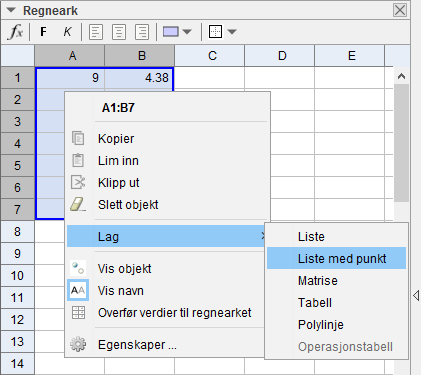
\includegraphics[width=0.475\linewidth]{figs/del2_2_geogebra}
		\caption{Skjermbilde av Geogebra til oppgave 2, del 2.}
		\label{fig:del22geogebra}
	\end{figure}
	
	
	# ``Skjæring mellom to objekt'' i Geogebra gir oss krysningspunktet mellom $f(x)$ og $g(x)$, som er $(91.6, 5.7)$.
	Ifølge modellen vil kvinner løpe like raskt som menn i år \answer{1991}.
	Se gjerne figur \ref{fig:del22modeller} for en graf som viser data og modeller.
	
	
	\begin{figure}[th!]
		\centering
		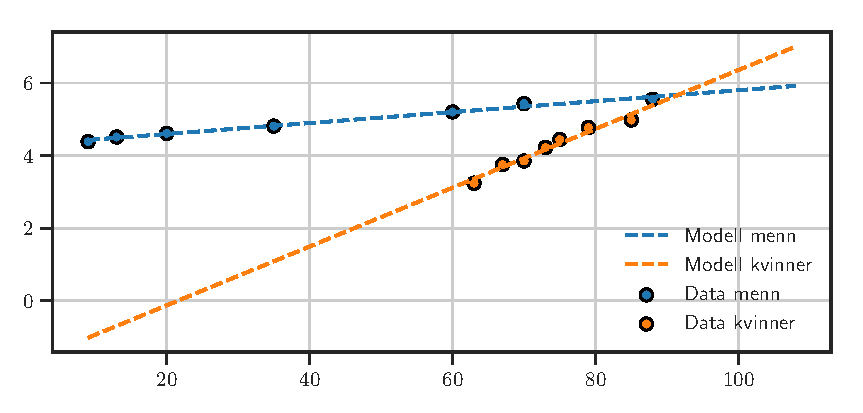
\includegraphics[width=0.7\linewidth]{figs/del2_2_modeller}
		\caption{Data og lineære modeller i oppgave 2, del 2.}
		\label{fig:del22modeller}
	\end{figure}
	
	# Spørsmål som dette er alltid litt skumle. Vi må formulere oss på en god måte.
	Gyldigheten er god i den forstand at linjene passer godt til punktene.
	Gyldigheten er dårlig i den forstand at prognosen for fremtiden ikke stemmer godt med
	hvordan utviklingen faktisk gikk, spesielt for kvinnene. 
	Dette er ofte tilfelle for lineære modeller---de fungerer bra innenfor visse områder, men man må være forsiktig dersom man ekstrapolerer\footnote{Å \emph{ekstrapolere} er å estimere utenfor datapunktene. Å \emph{interpolere} er å estimere innenfor datapunktene.}.
	For å undersøke litt mer nøyaktig kan vi regne ut den relative feilen når vi vet at modellenes anslag er $f(114) = 6.009$ og $g(114) = 7.487$.
	\begin{equation*}
		\text{relativ feil} = \frac{| \text{faktisk verdi} - \text{modellens anslag}|}{|\text{faktisk verdi}|}
	\end{equation*}
	Vi får følgende, der RF står for ``relativ feil.''
	\begin{equation*}
		\text{RF}_{\text{menn}} = \frac{|5.72 - 6.009|}{|5.72|} \approx 0.05 \quad 
		\text{RF}_{\text{kvinner}} = \frac{|5.01 - 7.487|}{|5.01|} \approx 0.49
	\end{equation*}
	Fra dette ser vi at den relative feilen for kvinner er mye høyere enn for menn. 
	Vi setter opp en tabell som undersøker over hvilken tidsperiode data er hentet fra,
	og hvor mange år det ekstrapoleres frem i tid.
	\begin{center}
		\begin{tabular}{l|lll}
		&	\textbf{Tidsperiode for data} & \textbf{Antall år ekstrapolert} & \textbf{Relativ} \\ \hline
		\textbf{Menn} &	80 år & 26 år ekstrapolert & $32.5\%$ \\
		\textbf{Kvinner} &	23 år & 29 år ekstrapolert & $126.1\%$ 
		\end{tabular}
	\end{center}
	Konklusjonen er at modellens gyldighet, i den grad den spådde fremtiden, var dårlig for kvinner.
	Mulige grunner er lite data og grov ekstrapolering---å spå hva som skjer om 29 år basert på 23 år med data er ikke særlig fornuftig.
	
	
	# Farten er gitt i meter per sekund. Farten som kreves for å løpe 42195 meter på 2 timer blir
	\begin{equation*}
		v = \frac{42195\text{ m}}{2 \times 3600 \text{ m}} = 5.86 \text{ m/s}
	\end{equation*}
	Vi bruker modellen
	\begin{equation*}
		h(x) = \frac{6.65}{1 + 0.751e^{-0.012x}}
	\end{equation*}
	og Geogebra til å regne ut $x^*$ slik at $h(x^*) = v$. 
	Vi lager grafen til modellen og linjen $y = 5.86$, og bruker deretter ``skjæring mellom to objekt.''
	Vi får da svaret $x^* = 143.18$. Menn vil i følge modellen springe maraton under 2 timer i år \answer{2043}.
	
	


\end{easylist}

\subsection*{Oppgave 3}
\begin{easylist}[enumerate]
	\ListProperties(Style2*=,Numbers=a,Numbers1=l,FinalMark={)})
	# Dersom fondet aldri skal gå tomt kan vi maksimalt dele ut overskuddet hvert år.
	Overskuddet blir $50 \text{ mill} \times 0.1 = 5 \text{ mill}$, fondet kan altså maksimalt dele ut \answer{5 millioner} kroner hvert år.
	
	# Vi antar her at vi får renter \emph{før} vi gjør utbetalingen etter det første året. 
	Vi kan undersøke problemstillingen ved hjelp av en tabell.
	Vi lar $S = 50$ være startbeløpet, $b = 8$ være beløpet som vi tar ut hvert år og $r = 1.1$ være rentefaktoren.
	Da får vi følgende mønster :
	\begin{center}
		\begin{tabular}{cl}
			\textbf{År} & \textbf{Penger} \\ \hline
			0 & $S$ \\
			1 & $Sr - b$ \\
			2 & $Sr^2 - br - b$ \\
			3 & $Sr^3 - br^2 - br - b$ \\
			$\vdots$ & $\vdots$ \\
			$n$ & $Sr^n - b \left( 1 + r + r^2 + \dots + r^{n-1}\right)$
		\end{tabular}
	\end{center}
	Vi må finne ut når pengene blir lik null, vi får likningen:
	\begin{align*}
		Sr^n &- b \left( 1 + r + r^2 + \dots + r^{n-1}\right) = 0 \\
		Sr^n &= b \sum_{i=0}^{n-1} r^i
	\end{align*}
	Denne løser vi i CAS i Geogebra slik: \\
	\texttt{NLøs[\{50*1.1\textasciicircum n = 8*Sum[1.1\textasciicircum i, i, 0, n-1]\}, \{n\}]} \\
	Løsningen blir $n \approx 10.29$. Fondet går tomt omtrent \answer{10 år etter 1. januar 2015},
	altså i 2025.29 $\approx$ april 2025. Siste store utbetaling blir i slutten av 2024.
	Se figur \ref{fig:del23plot} for en graf som viser situasjonen.
	
	
\begin{figure}[th!]
	\centering
	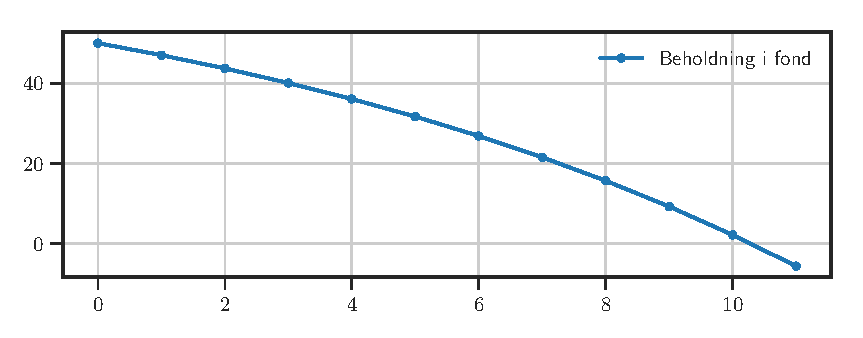
\includegraphics[width=0.7\linewidth]{figs/del2_3_plot}
	\caption{Fondet i oppgave 3, del 2.}
	\label{fig:del23plot}
\end{figure}
\end{easylist}

\subsection*{Oppgave 4}
La oss bruke variabelnavn som gir litt mening: $f$ er kilojoule per gram fett, $k$ er kilojoule per gram karbohydrater og $p$ er kilojoule per gram proteiner. For å løse likningssystemet skriver vi inn følgende i CAS i Geogebra. \\
\texttt{
Nløs[\{25*f + 2*k + 6*p = 1010,\\ 
3.5*f + 4.5*k + 3.3*p = 270, \\
27*f + 0*k + 27*p = 1500\},\\
\{f, k, p\}]} \\
Vi får da løsningen \answer{$f = 33.74$, $k=17.76$ og $p = 21.81$}.
Enheten blir kJ per gram.
Dette stemmer med likningssystemet, men ikke med virkeligheten---og med den kommentaren er vi ferdig med eksamen i matematikk.
	
	
\end{document}


